\section{Pure approach}

\subsection{Ground truth}
Real eBay auctions were collected by the API to generate the ground truth for the crowdsourcing experiments. The online auction platform divides their items in eight main categories: Motors, Fashion, Electronics, Collectibles \& Arts, Home \& Garden, Sporting Goods, Toys \& Hobbies and Deals \& Gifts. The ground truth consists of seven items from every category with the exception of the Motor's and Deals \& Gits sections, because the API can't search for items in these categories. First, some keywords were created to touch the desired category: ''Swiss Watch'' (Fashion), ''Smartphone'' (Electronics), ''Football Trading Card'' (Collectibles), ''Coffee Machine'' (Home), ''Soccer shoes'' (Sporting Goods), ''Action Figure'' (Toys) and ''Handbag'' (Fashion). The goal was also to have gender specific and neutral items. An action figure is used by male persons normally, the handbag by females and a smartphone by both. The Finding eBay API provides the method \textit{findCompletedItems} which takes keywords as a parameter and returns a list of completed auction items. The Python script search for the first sold item which uses US dollar as currency, has a description longer than one-hundred characters and contains of at least three images. Only three images were kept, because most of the auctions present the items with a top, front and side view. Another reason is the clarity for the crowdsourcing tasks. Every ground truth entry has the attributes title, description, category, condition, price and image one to three. The following table represents the final ground truth for the further experiments:
\begin{longtable}{| l | l | l | l |}
	\hline
	ID & Image 1 & Image 2 & Image 3 \\
	\hline
	\multirow{6}{*}{1} & 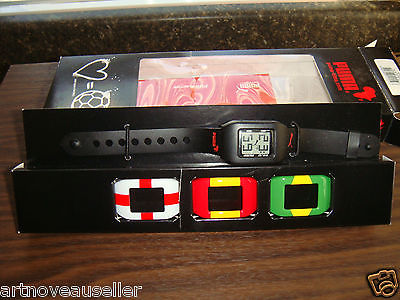
\includegraphics[scale=0.25]{images/ground_truth/1/image_1} & 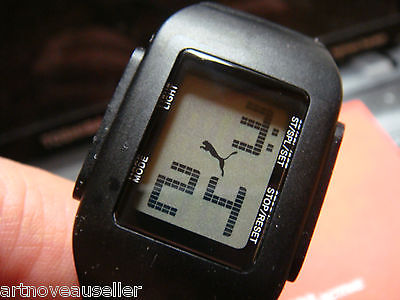
\includegraphics[scale=0.25]{images/ground_truth/1/image_2} & 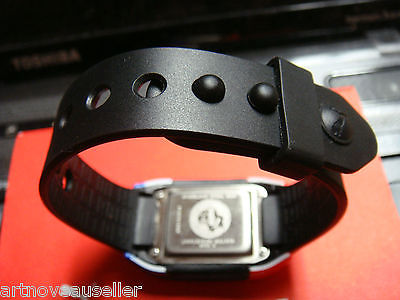
\includegraphics[scale=0.25]{images/ground_truth/1/image_3} \\
	\cline{2-4}
	\multirow{6}{*}{} & Title &  \multicolumn{2}{| p{10cm} |}{NIB 45 EURO \$\$ PUMA SPORT WRISTWATCH SWISS WATCH MOVEMENT LOVE+FOOTBALL} \\
	\cline{2-4}
	\multirow{6}{*}{} & Description &  \multicolumn{2}{| p{10cm} |}{ITEM IS BRAND NEW, FROM THE FIFA WORLD (MUNDIAL) FOOTBALL GAMES. WATCH HAS THREE INTERCHANGEABLE TOP COVER , EACH ONE REPRESENTING THE FLAG OF A TEAM PLAYING AT THE FIFA WORLD (MUNDIAL) FOOTBALL GAME PLUS ONE BLACK COVER IF YOU DON'T WISH TO WEAR THE FLAG COLORS INCLUDED IN THE PACKAGE AS SHOWN IN MY PICTURES. ITEM IS BRAND NEW NEVER USED WITH ORIGINAL BOX PAPERS AND INSTRUCTION ON HOW TO USE THIS WATCH.GREAT GIFT IDEA OR GREAT WATCH FOR THE SPORT LOVERS.ITEM COMES WITH WARRANTY FOR 90 DAYS FROM US AND MANUFACTURER WARRANTY OF 2 YEARS IS INCLUDED IN THE BOX.INSTRUCTIONS ARE IN DUTCH,ENGLISH,FRENCH,ITALIAN, CZECH,GERMAN, PORTUGUESE,SPANISH,HUNGARIAN,CHINESE AND JAPANESE.} \\
	\cline{2-4}
	\multirow{6}{*}{} & Category &  \multicolumn{2}{| p{10cm} |}{Jewelry \& Watches:Watches:Wristwatches} \\
	\cline{2-4}
	\multirow{6}{*}{} & Condition &  \multicolumn{2}{| p{10cm} |}{New with tags} \\
	\cline{2-4}
	\multirow{6}{*}{} & Price &  \multicolumn{2}{| p{10cm} |}{4.99} \\
	\hline \hline
	ID & Image 1 & Image 2 & Image 3 \\
	\hline
	\multirow{6}{*}{2} & 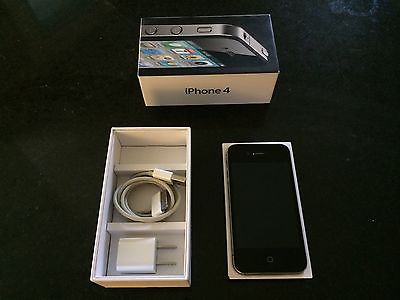
\includegraphics[scale=0.25]{images/ground_truth/2/image_1} & 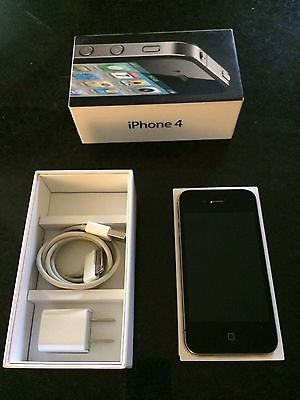
\includegraphics[scale=0.25]{images/ground_truth/2/image_2} & 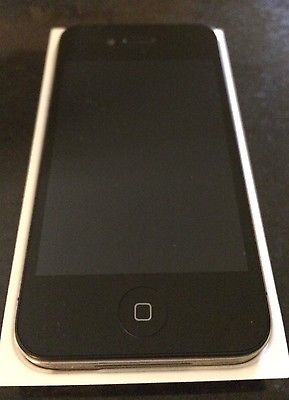
\includegraphics[scale=0.25]{images/ground_truth/2/image_3} \\
	\cline{2-4}
	\multirow{6}{*}{} & Title &  \multicolumn{2}{| p{10cm} |}{Apple iPhone 4 - 16GB - Black (Unlocked) Smartphone} \\
	\cline{2-4}
	\multirow{6}{*}{} & Description &  \multicolumn{2}{| p{10cm} |}{16GB Black iPhone 4, unlocked by carrier. This was an AT\&T phone so it is GSM, can be used internationally. This phone was manufacturer refurbished and then only used for about a week, so it is basically in perfect condition. Includes original packaging, 30-pin USB connector and charger.} \\
	\cline{2-4}
	\multirow{6}{*}{} & Category &  \multicolumn{2}{| p{10cm} |}{Cell Phones \& Accessories:Cell Phones \& Smartphones} \\
	\cline{2-4}
	\multirow{6}{*}{} & Condition &  \multicolumn{2}{| p{10cm} |}{Used} \\
	\cline{2-4}
	\multirow{6}{*}{} & Price &  \multicolumn{2}{| p{10cm} |}{185.0} \\
	\hline \hline
	ID & Image 1 & Image 2 & Image 3 \\
	\hline
	\multirow{6}{*}{3} & 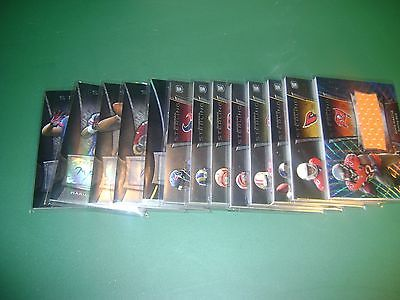
\includegraphics[scale=0.25]{images/ground_truth/3/image_1} & 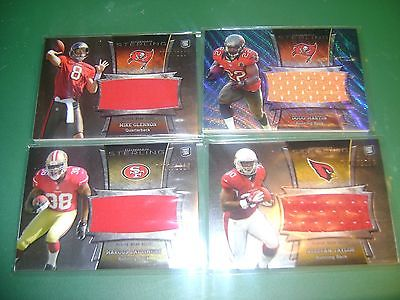
\includegraphics[scale=0.25]{images/ground_truth/3/image_2} & 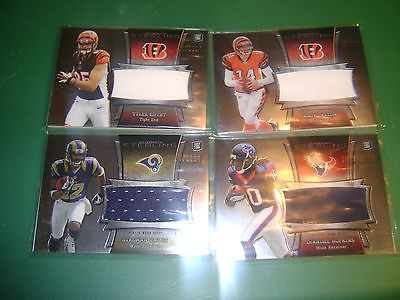
\includegraphics[scale=0.25]{images/ground_truth/3/image_3} \\
	\cline{2-4}
	\multirow{6}{*}{} & Title &  \multicolumn{2}{| p{10cm} |}{Lot of (13) 2013 Bowman Sterling Autograph Auto Relic Jersey Games Used} \\
	\cline{2-4}
	\multirow{6}{*}{} & Description &  \multicolumn{2}{| p{10cm} |}{This is for a 2013 Bowman Sterling Lot of 13 Game Used Relics and Autos. You get the exact cards that you see in the pictures. PLEASE PAY BY PAYPAL WITHIN 24 HOURS OF AUCTIONS END OR ITEM WILL BE RELISTED. S+H IS 3.99 WITH DELIVERY CONFIRMATION PLEASE CHECK OUT MY OTHER AUCTIONS} \\
	\cline{2-4}
	\multirow{6}{*}{} & Category &  \multicolumn{2}{| p{10cm} |}{Sports Mem, Cards \& Fan Shop:Cards:Football} \\
	\cline{2-4}
	\multirow{6}{*}{} & Condition &  \multicolumn{2}{| p{10cm} |}{Brand New} \\
	\cline{2-4}
	\multirow{6}{*}{} & Price &  \multicolumn{2}{| p{10cm} |}{27.0} \\
	\hline \hline
	ID & Image 1 & Image 2 & Image 3 \\
	\hline
	\multirow{6}{*}{4} & 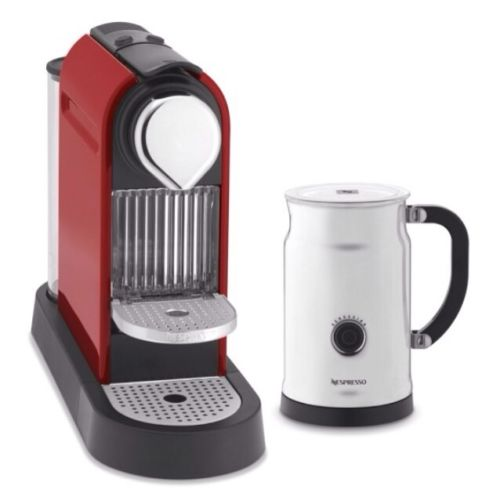
\includegraphics[scale=0.25]{images/ground_truth/4/image_1} & 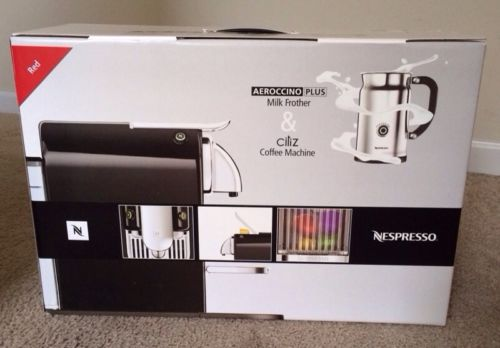
\includegraphics[scale=0.25]{images/ground_truth/4/image_2} & 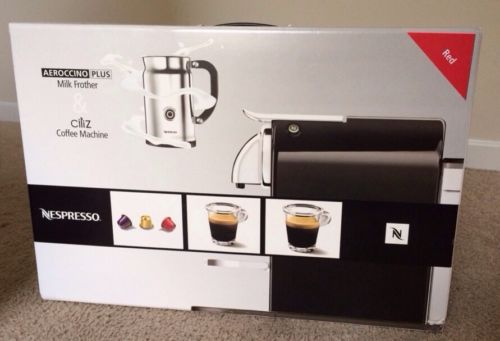
\includegraphics[scale=0.25]{images/ground_truth/4/image_3} \\
	\cline{2-4}
	\multirow{6}{*}{} & Title &  \multicolumn{2}{| p{10cm} |}{Nespresso Aeroccino Plus \& Citiz Coffee Machine {Red}} \\
	\cline{2-4}
	\multirow{6}{*}{} & Description &  \multicolumn{2}{| p{10cm} |}{Nespeesso Aeroccino Plus \& Citiz Coffee Machine Fully automatic brewing and milk frothing in two sleek, compact units. Works exclusively with Nespresso's premium coffee capsules, which are easy to order for delivery within two business days (for details, visit www.nespresso.com). Innovative Thermoblock technology with stainless-steel heating element guarantees precise temperature control. A 19-bar pressure pump ensures maximum extraction of flavor. Adjustable tray accommodates cups of various sizes (from small mug to travel cup). Removable water tank for easy refilling. Energy-save mode gradually reduces power if unit is left on. Includes Aeroccino Plus milk frother, which quickly heats milk for consistently perfect foam. Frother has two whisk attachments and an auto shutoff feature. Espresso maker: ABS plastic housing. 14 1/2" x 5" x 11" high. 34-fl.-oz.-cap. water tank. 10 lb. 1200W. Milk frother: Stainless-steel and plastic construction. 4" diam., 6-3/4" high. 8-oz. cap. 550W. This product is intended for use in the United States and Canada and is built to United States electrical standards. Posted with eBay Mobile} \\
	\cline{2-4}
	\multirow{6}{*}{} & Category &  \multicolumn{2}{| p{10cm} |}{Home \& Garden:Kitchen, Dining \& Bar:Small Kitchen Appliances:Coffee \& Tea Makers:Espresso Machines} \\
	\cline{2-4}
	\multirow{6}{*}{} & Condition &  \multicolumn{2}{| p{10cm} |}{New} \\
	\cline{2-4}
	\multirow{6}{*}{} & Price &  \multicolumn{2}{| p{10cm} |}{201.0} \\
	\hline \hline
	ID & Image 1 & Image 2 & Image 3 \\
	\hline
	\multirow{6}{*}{5} & 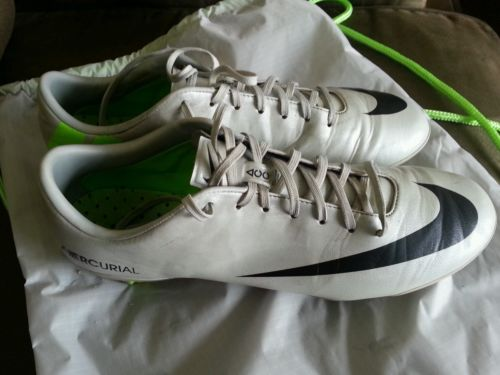
\includegraphics[scale=0.25]{images/ground_truth/5/image_1} & 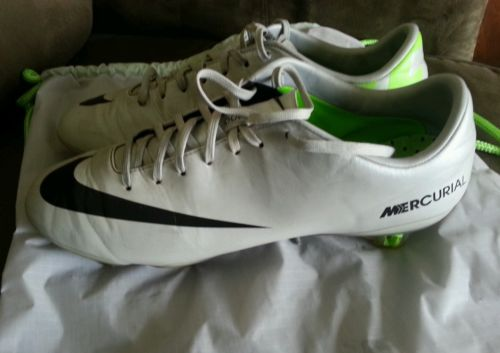
\includegraphics[scale=0.25]{images/ground_truth/5/image_2} & 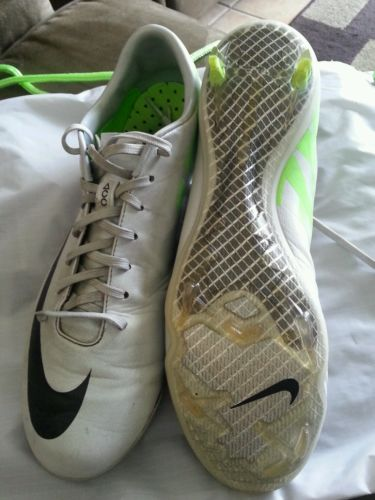
\includegraphics[scale=0.25]{images/ground_truth/5/image_3} \\
	\cline{2-4}
	\multirow{6}{*}{} & Title &  \multicolumn{2}{| p{10cm} |}{Nike Mercurial Vapor IX FG - Soccer Shoes Cleats - Metallic Platinum} \\
	\cline{2-4}
	\multirow{6}{*}{} & Description &  \multicolumn{2}{| p{10cm} |}{This is a pair of used Nike Vapor IX. They come with the string bag. In overall good condition with some signs of use. Clean and no smells. Mens size 7.5. Shipping is \$10.00 and includes tracking. I accept PayPal for payment.} \\
	\cline{2-4}
	\multirow{6}{*}{} & Category &  \multicolumn{2}{| p{10cm} |}{Sporting Goods:Team Sports:Soccer:Clothing, Shoes \& Accessories:Shoes \& Cleats:Men} \\
	\cline{2-4}
	\multirow{6}{*}{} & Condition &  \multicolumn{2}{| p{10cm} |}{Pre-owned} \\
	\cline{2-4}
	\multirow{6}{*}{} & Price &  \multicolumn{2}{| p{10cm} |}{76.99} \\
	\hline \hline
	ID & Image 1 & Image 2 & Image 3 \\
	\hline
	\multirow{6}{*}{6} & 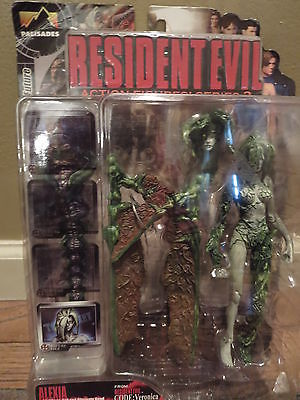
\includegraphics[scale=0.75]{images/ground_truth/6/image_1} & 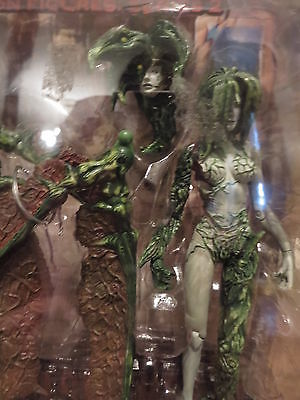
\includegraphics[scale=0.75]{images/ground_truth/6/image_2} & 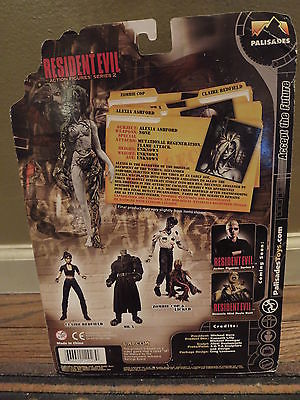
\includegraphics[scale=0.75]{images/ground_truth/6/image_3} \\
	\cline{2-4}
	\multirow{6}{*}{} & Title &  \multicolumn{2}{| p{10cm} |}{RARE Series 2 Palisades Resident Evil Code Veronica Alexia Action Figure} \\
	\cline{2-4}
	\multirow{6}{*}{} & Description &  \multicolumn{2}{| p{10cm} |}{This RARE and HARD TO FIND action figure will make and AWESOME collectable for any Resident Evil fan! This specific figure is part of the Resident Evil Code Veronica series. Alexia comes complete with Wings, Tail and Alternate Head to Transform into Alexia III and Logo Base. Great item for any RE fan!!! This item is still in its original packaging, unopened and unused. There is very slight wear around the cardboard edging from years of storage and a little adhesive residue on the plastic, most likely from a price sticker. Overall this item is in excellent condition!} \\
	\cline{2-4}
	\multirow{6}{*}{} & Category &  \multicolumn{2}{| p{10cm} |}{Toys \& Hobbies:Action Figures:TV, Movie \& Video Games} \\
	\cline{2-4}
	\multirow{6}{*}{} & Condition &  \multicolumn{2}{| p{10cm} |}{New} \\
	\cline{2-4}
	\multirow{6}{*}{} & Price &  \multicolumn{2}{| p{10cm} |}{90.0} \\
	\hline \hline
	ID & Image 1 & Image 2 & Image 3 \\
	\hline
	\multirow{6}{*}{7} & 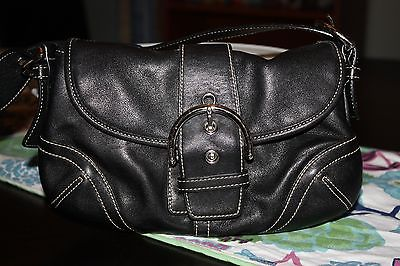
\includegraphics[scale=0.25]{images/ground_truth/7/image_1} & 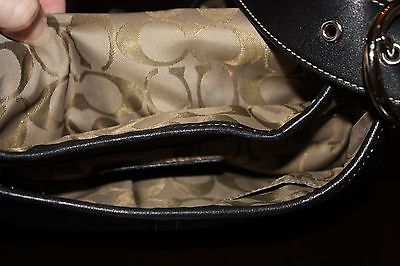
\includegraphics[scale=0.25]{images/ground_truth/7/image_2} & 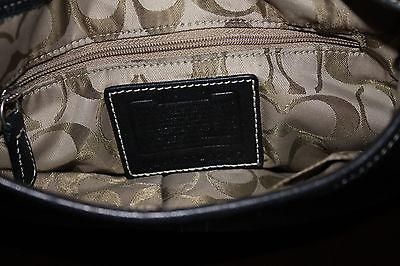
\includegraphics[scale=0.25]{images/ground_truth/7/image_3} \\
	\cline{2-4}
	\multirow{6}{*}{} & Title &  \multicolumn{2}{| p{10cm} |}{Black Coach purse leather GUC serial number H050-9247} \\
	\cline{2-4}
	\multirow{6}{*}{} & Description &  \multicolumn{2}{| p{10cm} |}{Pre-owned Black Coach hobo purse. GUC just because I did use it a couple of times. No stains,marks, or tears. Great condition!!!} \\
	\cline{2-4}
	\multirow{6}{*}{} & Category &  \multicolumn{2}{| p{10cm} |}{Clothing, Shoes \& Accessories:Women's Handbags \& Bags:Handbags \& Purses} \\
	\cline{2-4}
	\multirow{6}{*}{} & Condition &  \multicolumn{2}{| p{10cm} |}{Pre-owned} \\
	\cline{2-4}
	\multirow{6}{*}{} & Price &  \multicolumn{2}{| p{10cm} |}{35.0} \\
	\hline
\caption{Ground truth for pure crowdsourcing}
\end{longtable}
\subsection{Tasks workflow}
The inputs of the pipeline are images of the item to sell which were created by the seller. The images from the ground truth are used for the experiments of the thesis. To create item specific information for the auction, four subtasks were designed: 
\begin{itemize}
	\item Generate a title for the auction item
	\item Generate a description of the item
	\item Find one category for the auction item  
	\item Estimate the end price for the auction  
\end{itemize}
The digits in the brackets define the number of assignments. The seller receives at the end of the pipeline the information which he needs to create an auction on eBay. The starting price of the item depends on the sales strategy of the seller, but the end price should help to find a suitable one. The condition of the item, the auction duration or the payment settings have to be provided by the seller himself.
\begin{figure}[h!]
\centering
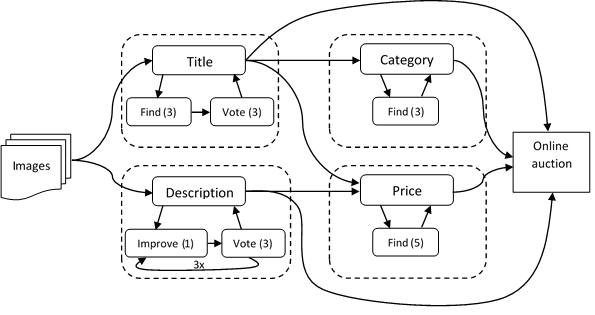
\includegraphics[scale=0.8]{images/pipelines/Pure_Pipeline.png}
\caption{Pure Crowdsourcing Pipeline}
\label{purePipeline}
\end{figure}

\subsection{Task design}
At the top of every HIT three images of an auction item are shown. Most of the sellers on eBay present their items with a front, side and top view. Only workers from the United States are allowed to participate in the created tasks, because the ground truth contains only items from there and they have a better feeling for the currency. Some of the tasks need a voting procedure to determine the final answer. The voters have to reason their votes mandatory to understand the strength of the selected answer. At the end of every task the contributors have the possibility to write down a feedback to the requestor.
\subsubsection{Title}
The goal of this subtask is to generate a clear and concise title for the auction item with at most eighty characters. The auction platform eBay provides some recommendations for a good title. It should contain the item's brand name, artist, or designer. A specification of the item could also be helpful. For example the title could include the size, color, condition, and model number. Correct spelling is a must. All these points will be presented to the worker in the instruction section of the task. To make the instructions clear, an example is also listed: 

Title: Sony Playstation 4 (black), 1 Controller, New 

After three titles were created by the crowd, the final title will be elected. If no title receive enough votes, the requester will act as an expert. The expert uses the search engine of the auction platform and decide which title shows more similar items. The Turkers will receive \$0.05 for finding a title and \$0.02 for voting.
\subsubsection{Description}
This subtask is a bit different then the others. An iterative task design is used. First, a worker creates an initial description of the item. Then, the second worker can improve the initial solution or create a new one. Then, the crowd decide which description should be kept and which one should be discarded. One iteration includes an improvement and a voting task. Three iterations were used to generate the description of the auction item. The workers should write approximately five sentences and include specific information like size, color, shape, age, manufacture date, company/author/artist, and notable features or markings. TurKit is a Java application to manage iterative approaches. For an improvement of the text a reward of \$0.2 will be paid, \$0.01 for every participant of the voting procedure.
\subsubsection{Category}
Based on the provided title, the workers have to find the most suitable eBay category for the auction item. The eBay search engine returns one or many categories for a given title. Then the worker has to decide which one matches best. For making a contribution, the workers achieve a payment of \$0.05.
\subsubsection{Price estimation}
The workers have to guess the end price of the online auction item in US dollar. Reasons for the estimation have to be mentioned additionally. The generated title and description are available for a better understanding of the picture contents. The workers have the possibility to list missing information for a more precise estimation. The participants receive a gratification of \$0.05.

Another idea to estimate the starting price is inspired by a German TV game show. The candidate has to predict the cost of an article. After the first guess, the game master answers with 'higher' or 'lower' until the right guess occur or the time is running out. If the player finds out the correct price then she/he will win the object.  
The idea of the show is modified to implement a game with a purpose, similar to the ESP game project \cite{esp}. The general procedure of the game is the following: 
\begin{enumerate}
	\item The system waits until two independent players are connected and ready to play 
	\item A few pictures, title and description of the article are displayed and the players had to read them first 
	\item Then the game starts and a first guess of the price will be shown by the system 
	\item Both users have to decide if the real price is higher or lower than the displayed one 
	\item Dependent on the previous response, the system will present a higher or lower price until the countdown is expired or there are no guesses left 
	\item The players will receive a score dependent on the difference of the price estimation. A smaller difference leads to a higher score, a higher one to a lower score 
\end{enumerate}
The first guess of the system will be the mean value \( \mu \) of a large number of sold items on eBay. The value can be determined by the eBay API. The guessing structure will be implemented as a directed binary tree. The root node represents the mean value and every following child node will have a lower (left child) \( v_l \) or higher (right child) value  \( v_r \), determined by the value of the parent node  \( v_p \) and the depth  \( d \) of the tree. The following formula calculates the values  of the nodes: 
\begin{equation}
v_l(v_p,d) = v_p - \frac{\mu}{2^d}
\end{equation}
\begin{equation}
v_r(v_p,d) = v_p + \frac{\mu}{2^d}
\end{equation}
The leafs are integer values which can't be divided by two and represents the final guess of a player. If the time is up and the guesser doesn't reach a leaf node, the value of the actual node is taken. 
The score of the price prediction is determined by a scoring function \( s \), where \( x_1 \) and \( x_2 \) are the price estimations of player 1 and 2.
\begin{equation}
s(x_1,x_2) = 1 - |\varphi(x_1) - \varphi(x_2)|
\end{equation}
The function \( \varphi \) is responsible to normalise the estimations (interval from 0 to 1).
\begin{equation}
\varphi(x) = \frac{x}{2\mu}
\end{equation}
The function is also used to weight the different estimations for the same product. If \( n \) rounds are played for a given object, the final price \( t \) is calculated:
\begin{equation}
t = \frac{1}{\sum_{k=1}^{n} s(x_{k1},x_{k2})}\left(\sum_{i=1}^{n} s(x_{i1},x_{i2})\frac{x_{i1}+x_{i2}}{2}\right)
\end{equation}
The reliability \( r \) of the price estimation is the mean score of all played games for the same object:
\begin{equation}
r = \frac{1}{n}\left(\sum_{i=1}^{n} s(x_{i1},x_{i2})\right)
\end{equation}

\subsection{Variations}
The prior section describes the standard composition of the tasks. To survey the behaviour of the workers, some design modifications were made: 
\subsubsection{Image Quantity and Quality}

All available images were presented to the crowd with the highest image resolution. The basis setting of the tasks shows only the first three images. The following table illustrates the number of additional images per item and the corresponding resolutions: 
\begin{table}[h!]
	\begin{center}
	\begin{tabular}{| l | l | l | p{10cm} |}
		\hline
		Ground Truth ID & Total Images & Normal Resolution (< 1600 x 1200) & High Resolution (1600 x 1200) \\
		\hline
		1 & 6 & 0 & 6 \\
		\hline
		2 & 3 & 3 & 0 \\
		\hline
		3 & 4 & 0 & 4 \\
		\hline
		4 & 7 & 7 & 0 \\
		\hline
		5 & 9 & 0 & 9 \\
		\hline
		6 & 3 & 0 & 3 \\
		\hline
		7 & 4 & 0 & 4 \\
		\hline
	\end{tabular}
	\end{center}
	\caption{}
\end{table}
\subsubsection{Market Price}
The actual market price of the items was mentioned in the price estimation task. The web service pricegrabber.com was used to find reliable and consistent prices. 
\begin{table}[h!]
	\begin{center}
	\begin{tabular}{| l | p{10cm} |}
		\hline
		Ground Truth ID & Price (in USD) \\
		\hline
		1 & 69.00 \\
		\hline
		2 & 399.99 \\
		\hline
		3 & 49.99 \\
		\hline
		4 & 299.00 \\
		\hline
		5 & 189.99 \\
		\hline
		6 & 44.99 \\
		\hline
		7 & 289.99 \\
		\hline
	\end{tabular}
	\end{center}
	\caption{}
\end{table}
\subsubsection{Commission}
This section describes the idea of an additional incentive for the workers which is added to the reward of MTurk tasks as a bonus. If an auction item will be sold successfully on eBay then all contributors of the crowdsourced result will receive a commission of the end price. The ground truth contains already completed eBay auctions and therefore the criterion of the bonus has to be determined otherwise. Only those created auctions which get more votes, during the evaluation process, than the ground truth will receive a commission. The table x.x shows the distribution of the percentages. The bonus can be between 2.55\% and 4.9\% of the end price. The range of the end prices in the ground truth goes from \$4.99 (watch) to \$201 (coffee machine). From this it follows that the commission can be between \$0.127 (2.55\% of \$4.99) and \$9.85 (4.9\% of \$201). The differences of the worker behaviour and a potential quality intensification will be investigated. 
\begin{table}[h!]
	\begin{center}
	\begin{tabular}{| l | l | l | p{10cm} |}
		\hline
		Name of task & Number of assignements (Min) & Number of assignements (Max) & Percentage of commission (in \%) \\
		\hline
		Title (Finding) & 1 & 1 & 0.25 \\
		\hline
		Title (Voting) & 2 & 3 & 0.1 \\
		\hline
		Description (Improving) & 1 & 1 & 1.0 \\
		\hline
		Description (Voting) & 2 & 2 & 0.05 \\
		\hline
		Category & 2 & 3 & 0.25 \\
		\hline
		Price & 1 & 5 & 0.5 \\
		\hline
		Total (Min) & & & 2.55 \\
		\hline
		Total (Max) & & & 4.9 \\
		\hline
	\end{tabular}
	\end{center}
	\caption{}
\end{table}

\subsubsection{Non-branded Item}
All of the ground truth items have visible brand labels. Some are more famous (Apple, Puma) than the others (Palisades, Powman Sterling). Information about the brands and their manufactured items can be found easily. Describing an unknown object is more difficult. A non-branded item is put into the pipeline to research the ability of the workers to handling such items.
\begin{table}[h!]
	\begin{center}
	\begin{tabular}{| l | l | l |}
	\hline
	Image 1 & Image 2 & Image 3 \\
	\hline
	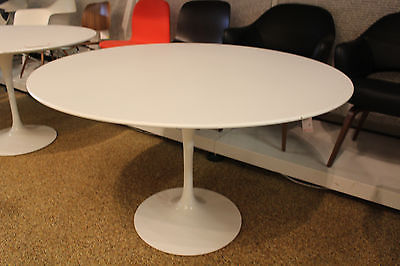
\includegraphics[scale=0.25]{images/ground_truth/8/image_1} & 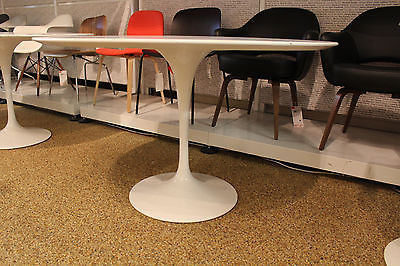
\includegraphics[scale=0.25]{images/ground_truth/8/image_2} & 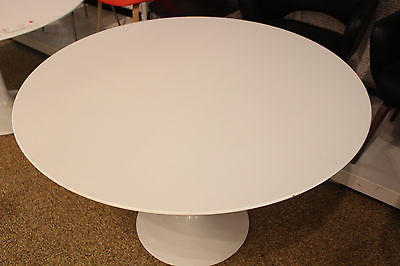
\includegraphics[scale=0.25]{images/ground_truth/8/image_3} \\
	\hline
	Title &  \multicolumn{2}{| p{10cm} |}{Saarinen Round Dining Table 47" White Laminate White Base KNOLL DWR} \\
	\hline
	Description &  \multicolumn{2}{| p{10cm} |}{Living Dining Outdoor Workspace Lighting Floor Accessories MidCentury Modern Saarinen Round Dining Table 47" (White Laminate/White Base) You are bidding on an AUTHENTIC Saarinen Round Dining Table, 47" in White Laminate with White base. Great condition, slight signs of handling. In a 1956 cover story in Time magazine, Eero Saarinen said he was designing a collection to "clear up the slum of legs in the U.S. home." Later that year, he completed his Pedestal Table and TulipTM Chair Collection (1956) and obliterated the "slum" by creating a cast aluminum base inspired by a drop of high-viscosity liquid. This table is manufactured by Knoll according to the original and exacting specifications of the designer. Made in Italy. Pedestal Tables come in a variety of table top materials (veneer, marble and laminate) and base colors (black, white and platinum).The base has an abrasion-resistant Rilsan finish.Each piece is stamped with the KnollStudio logo and Eero Saarinen's signature.Measurements: Assembled Table H 28.25" Diameter 47" Materials: Cast aluminum base with Rilsan finish; bevel-edged top in laminate Laminate: MDF with laminate.} \\
	\hline
	Category &  \multicolumn{2}{| p{10cm} |}{Home \& Garden:Furniture:Tables} \\
	\hline
	Condition &  \multicolumn{2}{| p{10cm} |}{Used} \\
	\hline
	Price &  \multicolumn{2}{| p{10cm} |}{1277.00} \\
	\hline
	\end{tabular}
	\end{center}
	\caption{}
\end{table} 

\section{Hybrid approach}
\subsection{Ground truth}
A lot of sold items were collected by the help of the eBay API. The used methods were the same as in the prior ground truth generation (Chapter x). After all the necessary data were collected, the Python script splits the data shuffled into a training and test set. The training set contains of 70 percent of the whole data. All the consecutively steps (data analysis, feature reduction) will use the training set until the performance of a classifier will be proved on the test set. The ground truth was generated for three different item types:
\begin{table}[h!]
	\begin{center}
	\begin{tabular}{| p{5cm} | l | l | l |}
		\hline
		Item type & Total number of auctions & Size of training set & Size of test set \\
		\hline
		Apple iPhone & 2299 & 1609 & 690 \\
		\hline
		Hot Wheels Cars, 1:64, Ford Mustang & 1045 & 731 & 314 \\
		\hline
		Sony Playstation & 943 & 660 & 283 \\
		\hline
	\end{tabular}
	\end{center}
	\caption{}
\end{table}
\subsection{Tasks workflow}
\subsection{Task design}
\subsubsection{Title}
\subsubsection{Description}
\subsubsection{Category}
\subsubsection{Price estimation}
\subsection{Pre-processing}
\subsection{Feature extraction}
\subsubsection{Item Specific Features}
\paragraph{Apple iPhone}
The iPhone made by Apple is available in eight models. The first generation was released in 2007, the last model 5s in 2013. Every model comes with different storage sizes (from 8GB to 64GB). The values for the condition property on eBay depend on the corresponding item category. All the values are nominal and will be converted to numerical.
\begin{table}[h!]
	\begin{center}
	\begin{tabular}{| l | p{5cm} | p{4cm} | l | l |}
		\hline
		Name & Description & Values & Range & Data type \\
		\hline
		Model & The model of the iPhone where 0 is the oldest generation and 7 the newest & 1st, 3G, 3GS, 4, 4S, 5, 5C, 5S & [0, 7] & Integer \\
		\hline
		Storage & The size of the storage of the smartphone & 8GB, 16GB, 32GB, 64GB & [1, 4] & Integer \\
		\hline
		Condition & The condition of the iPhone & New, New other, Manufacturer refurbished, Seller refurbished, Used, For parts or not working & [1, 6] & Integer \\
		\hline
	\end{tabular}
	\end{center}
	\caption{}
\end{table}

\paragraph{Mattel Hot Wheels Cars}
Mattel produces diecast car models in different sizes and series. Cars with a ratio of 1:64 are the most popular ones. The collected data contains only Ford Mustang cars, because they are very famous in the US and it should be possible to distinguish between different models. The exact model is indicated by a date.
\begin{table}[h!]
	\begin{center}
	\begin{tabular}{| l | p{5cm} | p{4cm} | l | l |}
		\hline
		Name & Description & Values & Range & Data type \\
		\hline
		Model & The model of the Ford Mustang where 1964 is the oldest and 2014 the newest & & [1964, 2014] & Integer \\
		\hline
		Condition & The condition of the car & New, Used & {1, 2} & Integer \\
		\hline
	\end{tabular}
	\end{center}
	\caption{}
\end{table}

\paragraph{Sony Playstation}
Sony's Playstation exists in ten versions. Two of them are portable and for the second and third model of the console is a slim version available. Every device has a region code or all data carriers are readable. There is no simple way to extract the storage size of the consoles at the moment, because eBay doesn't provide a field for this specific information.
\begin{table}[h!]
	\begin{center}
	\begin{tabular}{| l | p{5cm} | p{4cm} | l | l |}
		\hline
		Name & Description & Values & Range & Data type \\
		\hline
		Model & The model of the Playstation & 1, 2, 2 Slim, 3, 3 Slim, 4, Vita, Portable & [0, 7] & Integer \\
		\hline
		Region Code & The region code of the console & Not specified, NTSC, PAL, Region free & [0, 3] & Integer \\
		\hline
		Condition & The condition of the item & New, New other, Manufacturer refurbished, Seller refurbished, Used, For parts or not working & [1, 6] & Integer \\
		\hline
	\end{tabular}
	\end{center}
	\caption{}
\end{table}

\subsubsection{Auction Specific Features}
The auction itself is described by the features in this section. The list contains some timing and shipping information. Also the number of pictures and the description length could have an influence to the result of the auction. All values are numerical.
\begin{table}[h!]
	\begin{center}
	\begin{tabular}{| l | p{5cm} | l | l | l |}
		\hline
		Name & Description &  Range & Data type \\
		\hline
		Duration & The duration of the auction in days & {1, 2, 3, 7, 10} & Integer \\
		\hline
		Number of pictures & Number of pictures attached to the auction & [1, 12] & Integer \\
		\hline
		Length of description & Length of the item description & [0, 500'000] & Integer \\
		\hline
		End weekday & The last weekday of the auction duration & [1, 7] & Integer \\
		\hline
		Start weekday & The weekday of the creation date & [1, 7] & Integer \\
		\hline
		End hour & At what hour the auction was ended & [0, 23] & Integer \\
		\hline
		Global shipping & The item will be shipped over the whole world or not & {0, 1} & Boolean \\
		\hline
		Shipping locations & The number of countries where the item will be shipped & [0, 249] & Integer \\
		\hline
		Shipping type & Specifies the calculation of the shipping costs & [0, 7] & Integer \\
		\hline
		Returns accepted & If the buyer can return the item or not & {0, 1} & Boolean \\
		\hline
		Handling time & How many days will it take until the item is put in the mail once the seller receive payment & {1, 2, 3, 4, 5, 10, 15, 20} & Integer \\
		\hline
	\end{tabular}
	\end{center}
	\caption{}
\end{table}
\subsubsection{Seller Specific Features}
These features characterise the seller who created the auction. Every user on eBay has the possibility to give a positive, neutral or negative feedback after every transaction. The rating system awards stars with twelve different colors for trustful sellers. After ten positive feedbacks the user receives a yellow star for example. Therefore, the nominal value has to be converted to an integer.
\begin{table}[h!]
	\begin{center}
	\begin{tabular}{| l | l | l | l | l |}
		\hline
		Name & Description &  Range & Data type \\
		\hline
		Seller rating & Percentage of positive feedbacks & [0, 100] & Float \\
		\hline
		Seller rating count & Number of positive minus negative buyer feedbacks & [0, 12] & Integer \\
		\hline
	\end{tabular}
	\end{center}
	\caption{}
\end{table}
\subsection{Parameter Search}
\subsection{Cross-Validation}
\subsection{Signifigance Test}
\subsection{Classifiers}
